\begin{frame}
  \frametitle{The Planck Power Spectrum}
  \framesubtitle{A perfect fit}
  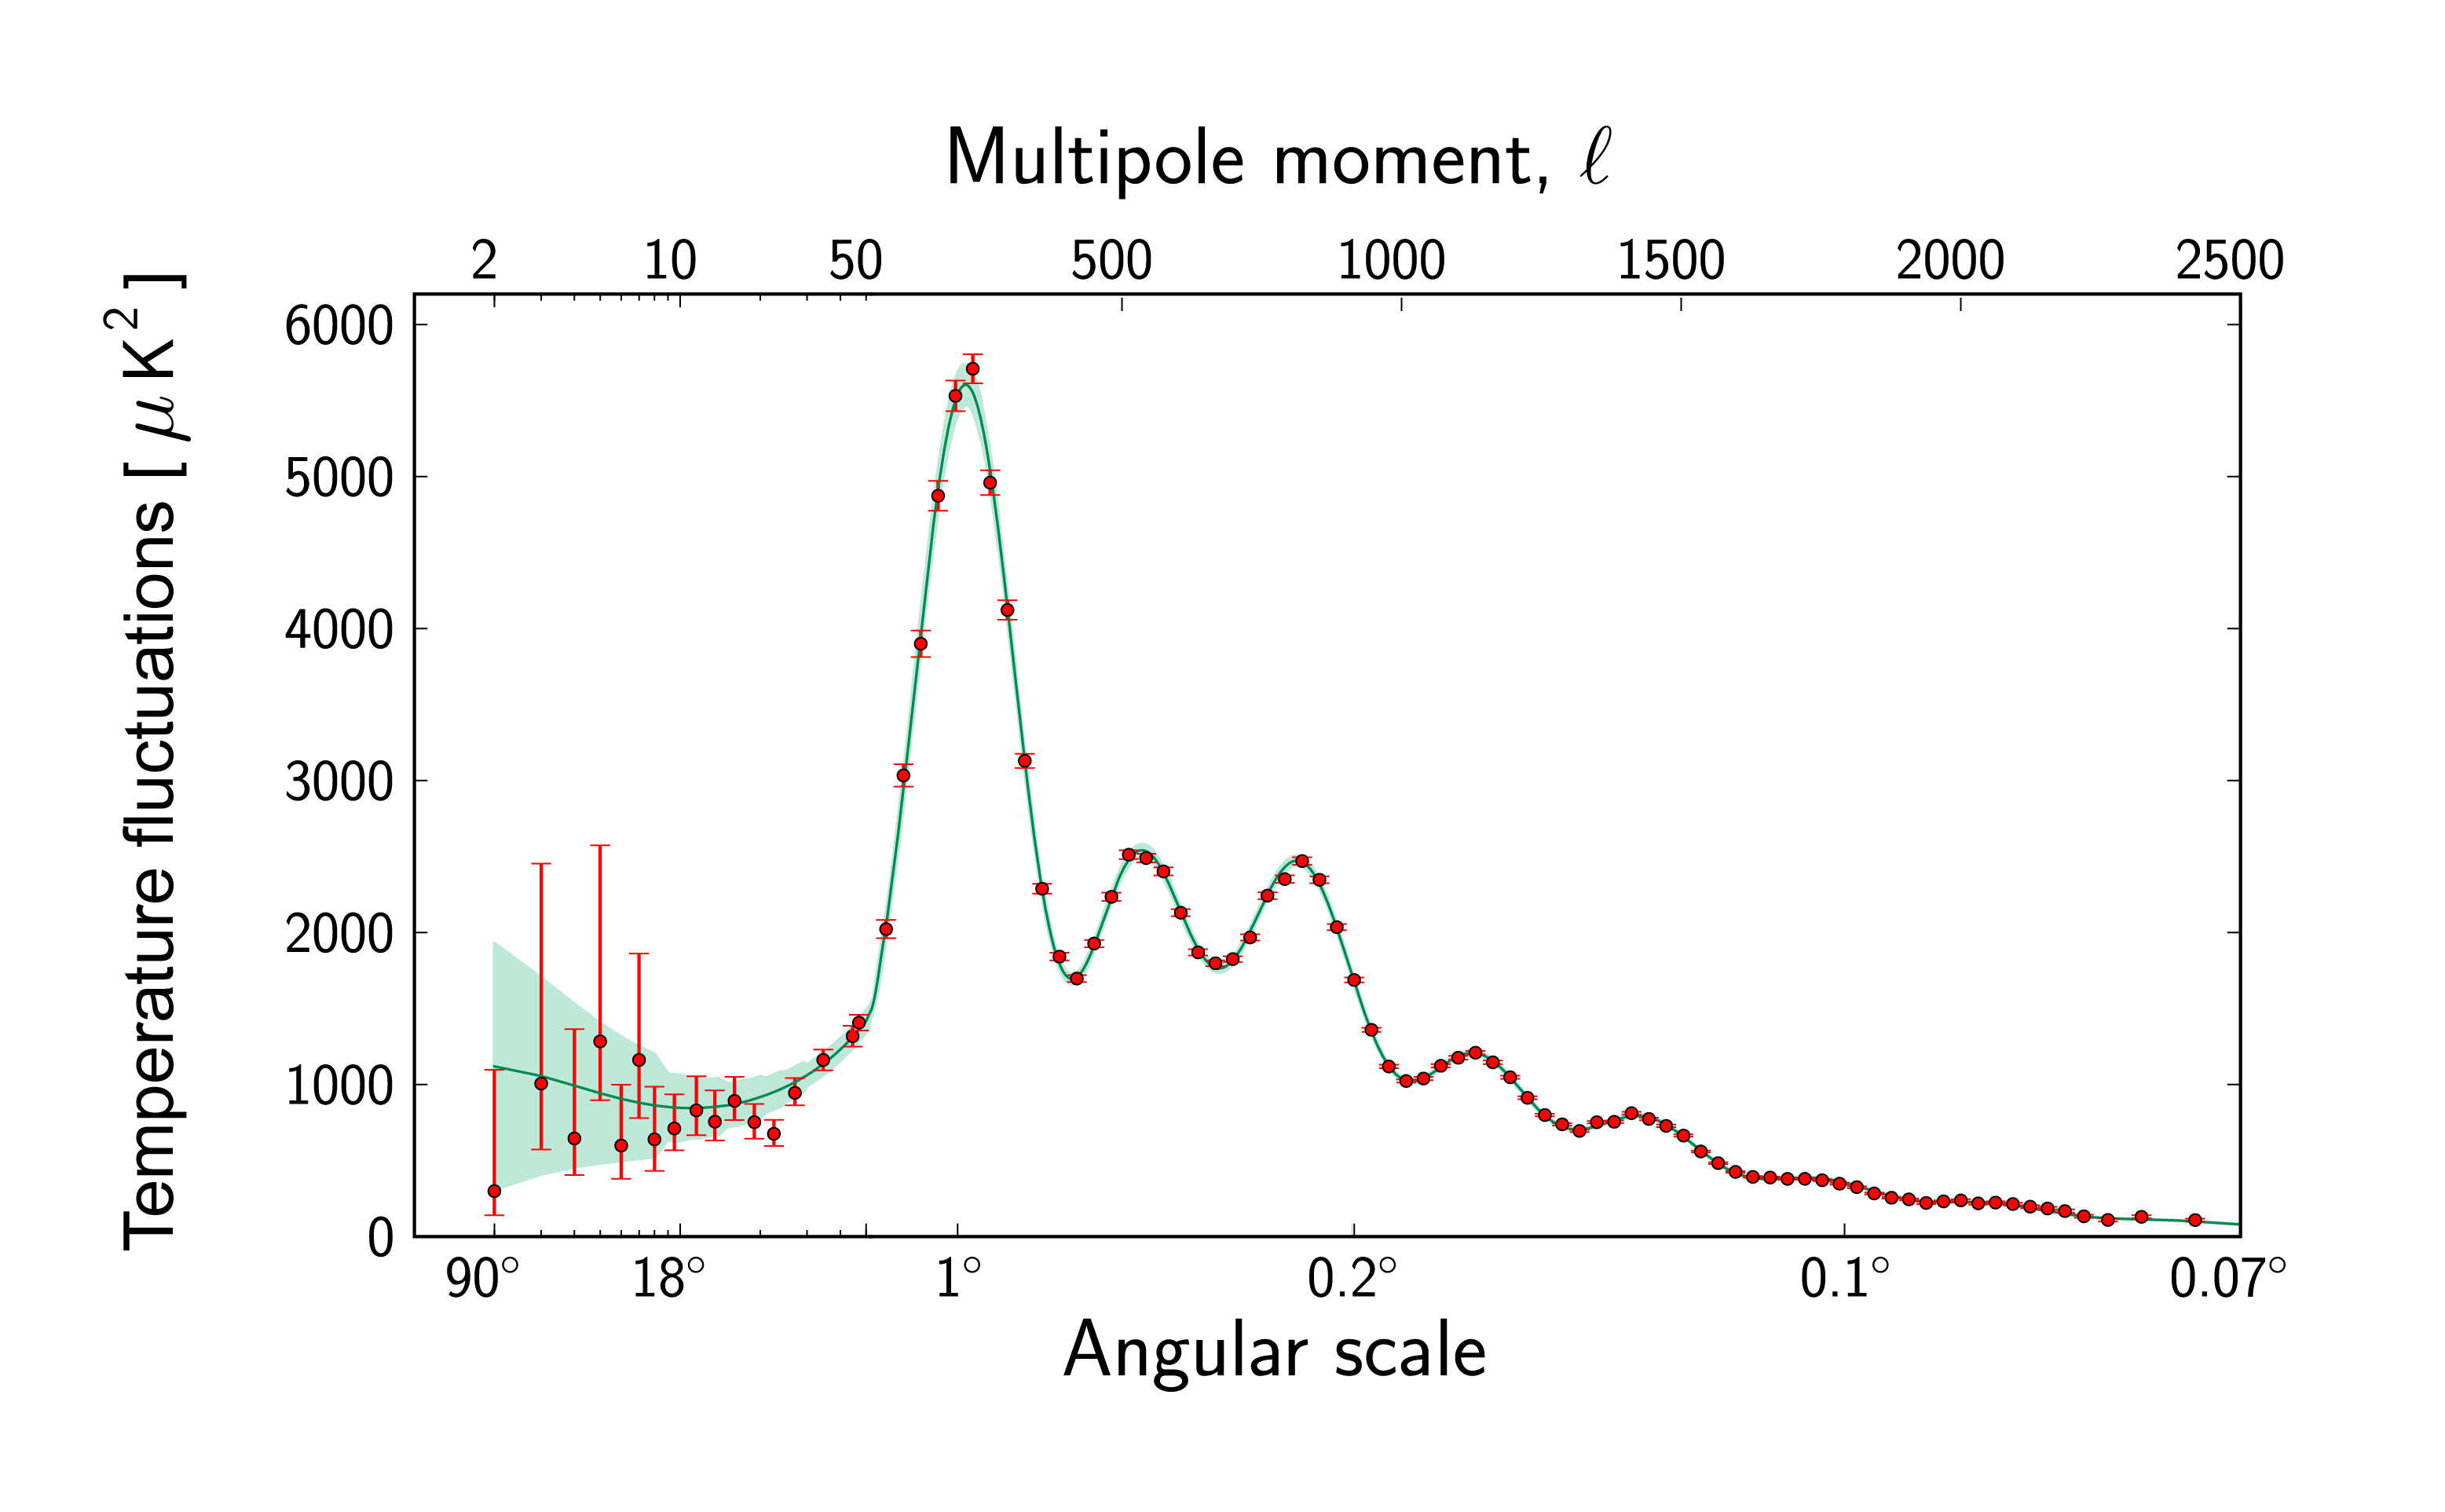
\includegraphics[width=\textwidth]{Images/planck_power_spec.jpg}
\end{frame}



\begin{frame}
  \frametitle{Explaining the wiggles}
  \framesubtitle{Inflation at its best}

  \makebox[\textwidth][c]{%
    \begin{tikzpicture}
      \begin{axis}[
          ytick=\empty,
          width=\textwidth,
          height=0.5\textheight,
          xmin=0,xmax=1800,
          ymin=-2,ymax=2,
          xtick={405,1080,1400},
          xticklabels={start,end,last scatter},
          domain=0:1800,
          xlabel={time},
          ylabel={perturbation}
        ]
        \only<1->{
          \addplot [domain=0:405,samples=500]{sin(2*x)}
        };
        \only<3->{
          \addplot [domain=405:1080,samples=500]{sin(2*405)}
        }; 
        \only<4->{
          \addplot [domain=1080:1800,samples=500]{cos(x)}
        }; 

        \only<5->{
          \addplot [domain=0:405,samples=500]{0.5*sin(2*x-45)} 
        };
        \only<5->{
          \addplot [domain=405:1080,samples=500]{0.5*sin(2*405-45)}
        }; 
        \only<5->{
          \addplot [domain=1080:1800,samples=500]{0.5*sin(2*405-45) * cos(x)}
        }; 
        \only<7->{
        \addplot [domain=0:405,samples=500]{0.75*sin(2*x-135)} 
        }; 
        \only<7->{
        \addplot [domain=405:1080,samples=500]{0.75*sin(2*405-135)} 
        }; 
        \only<7->{
        \addplot [domain=1080:1800,samples=500]{0.75*sin(2*405-135) * cos(x)} 
        }; 
        \only<7->{
        \addplot [domain=0:405,samples=500]{0.25*sin(2*x-225)} 
        }; 
        \only<7->{
        \addplot [domain=405:1080,samples=500]{0.25*sin(2*405-225)} 
        }; 
        \only<7->{
        \addplot [domain=1080:1800,samples=500]{0.25*sin(2*405-225) * cos(x)} 
        }; 

        \addplot [domain=-2:2,dash pattern=on 1pt off 2pt]({405},{x});
        \addplot [domain=-2:2,dash pattern=on 1pt off 2pt]({1080},{x});
        \addplot [domain=-2:2,dash pattern=on 1pt off 2pt]({1400},{x});

      \end{axis}
    \end{tikzpicture}
  }
\begin{itemize}
  \item<2-> Inflation acts to stretch perturbations
  \item<6-> Afterwards, perturbations come back in phase
  \item<8-> Last scattering surface records fixed time after inflation
  \item<9-> Different modes at surface will have different amplitudes
\end{itemize}


\end{frame}
